\subsubsection{Đường ống dữ liệu Pháp Điển}

Sơ đồ tổng quan Data pipeline Pháp Điển

\begin{figure}[H]
\centering
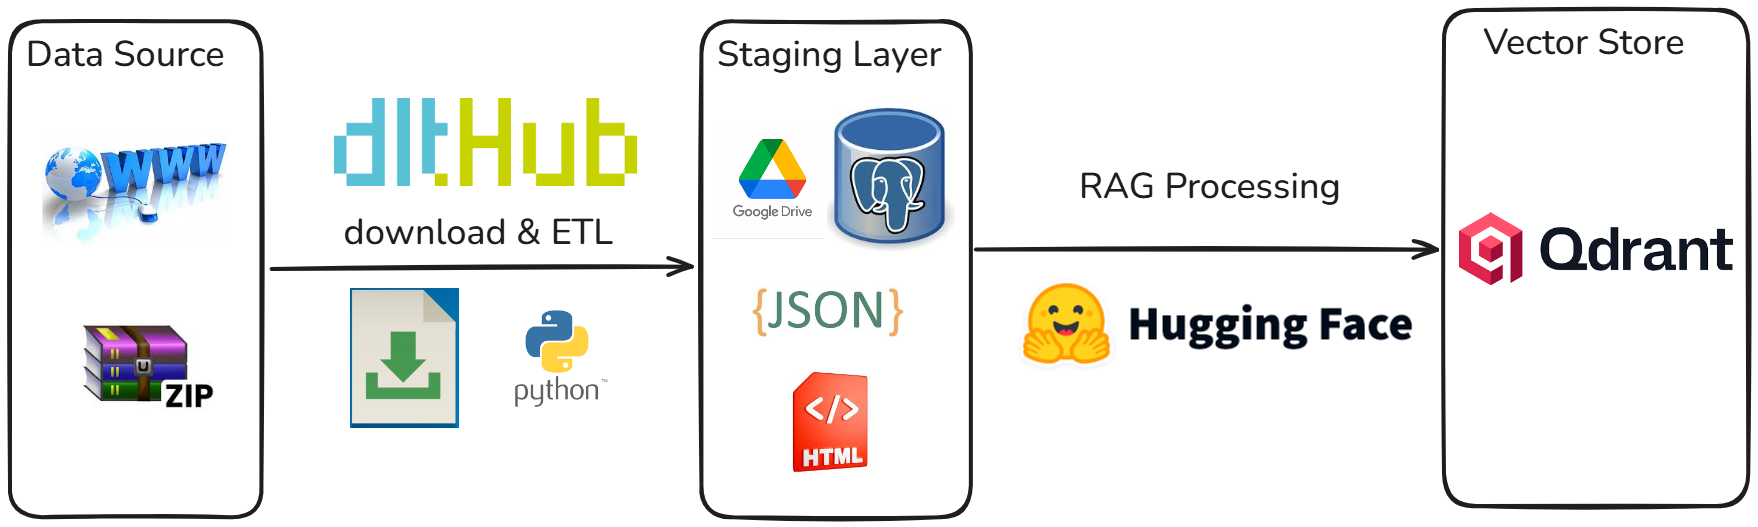
\includegraphics[width=0.99\textwidth]{pictures/Data-Pipeline-PhapDien.excalidraw.png}
\caption{Sơ đồ tổng quan luồng dữ liệu Pháp Điển}
\end{figure}

Tổng quan thông tin cấu trúc trong file ZIP

\begin{figure}[H]
\centering
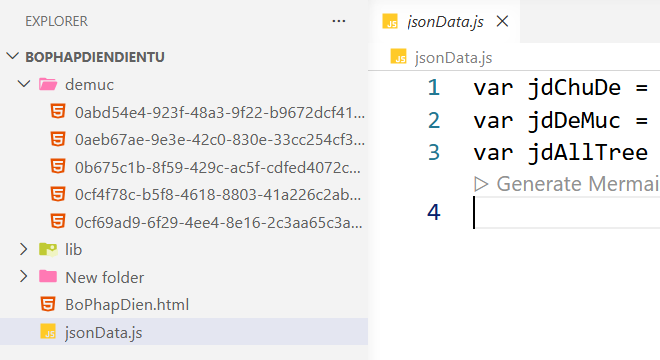
\includegraphics[width=0.75\textwidth]{pictures/zip_file_PhapDien-v2.png}
\caption{Tổng quan thông tin cấu trúc trong file ZIP}
\end{figure}

Kết quả folder và file JSON đã trích xuất trong Google Drive

\begin{figure}[H]
\centering
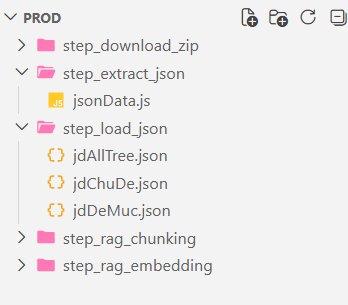
\includegraphics[width=0.6\textwidth]{pictures/step_json_PhapDien-v2.png}
\caption{Kết quả folder và file JSON đã trích xuất trong Google Drive}
\end{figure}

Kết quả vector được lưu trong vector database

\begin{figure}[H]
\centering
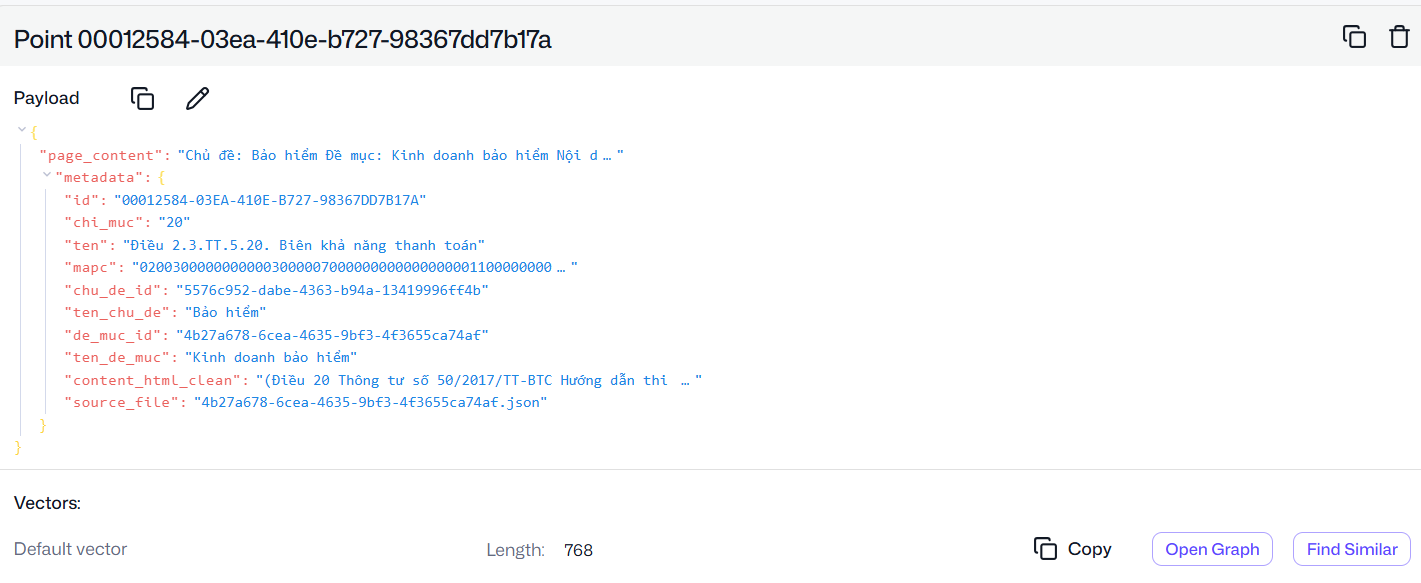
\includegraphics[width=0.95\textwidth]{pictures/vector_database_PhapDien-v2.png}
\caption{Kết quả vector được lưu trong vector database}
\end{figure}

% Các bước thực hiện

\begin{figure}[H]
\centering
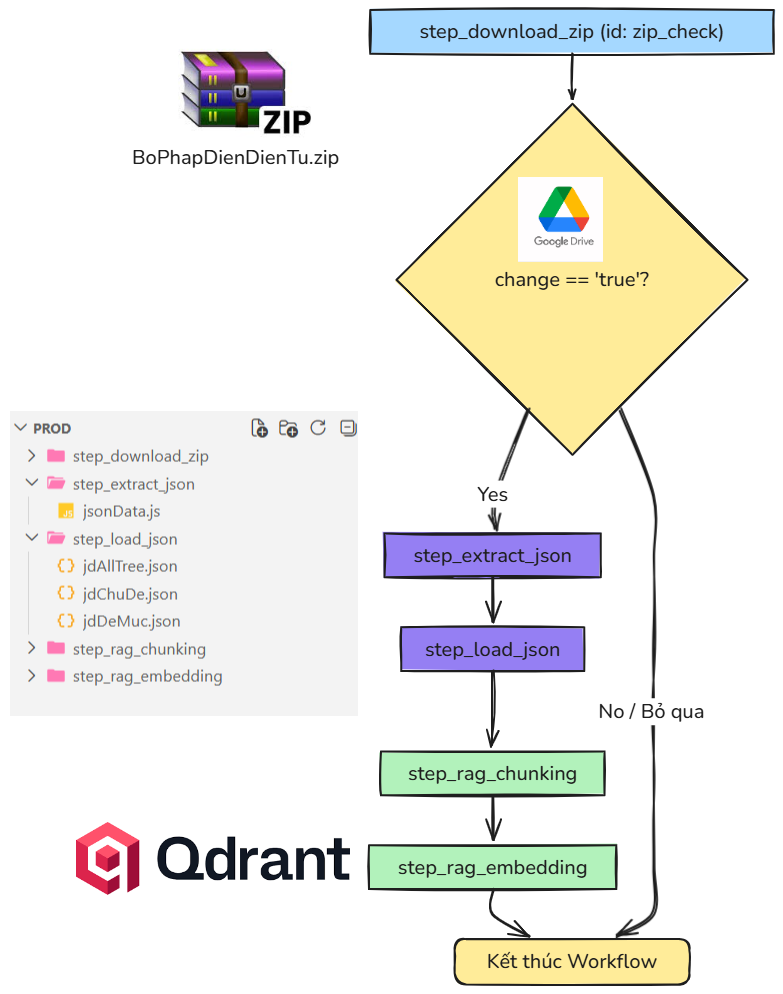
\includegraphics[width=0.4\textwidth]{pictures/step3.excalidraw.png}
\caption{Tổng quan các bước luồng dữ liệu Pháp Điển}
\end{figure}

% Mô tả các bước thực hiện:

Quá trình Data pipeline được chia thành 3 giai đoạn: Thu thập dữ liệu, tiền xử lý văn bản và tích hợp RAG Pipeline.

% \textbf{Giai đoạn Thu thập Dữ liệu:}
\begin{itemize}
\item \texttt{step\_download\_zip}:
Tự động tải file nén chứa toàn bộ Bộ Pháp Điển điện tử
% (\texttt{BoPhapDienDienTu.zip})
từ nguồn Cổng thông tin điện tử Pháp Điển. Hệ thống tính toán mã băm (MD5) và đồng bộ với Google Drive để kiểm tra sự thay đổi dữ liệu.

\begin{figure}[H]
\centering
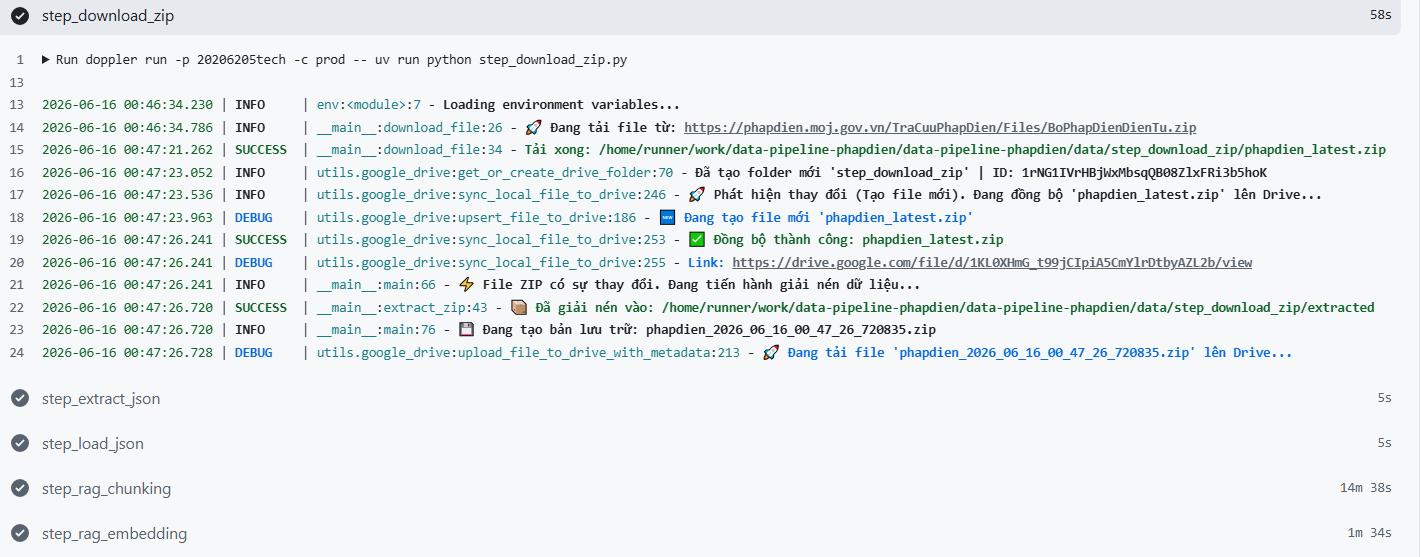
\includegraphics[width=0.85\textwidth]{pictures/data-pipeline-phapdien-step-download-zip-new.png}
\caption{Tự động tải file nén mới và đồng bộ Google Drive}
\end{figure}

\begin{figure}[H]
\centering
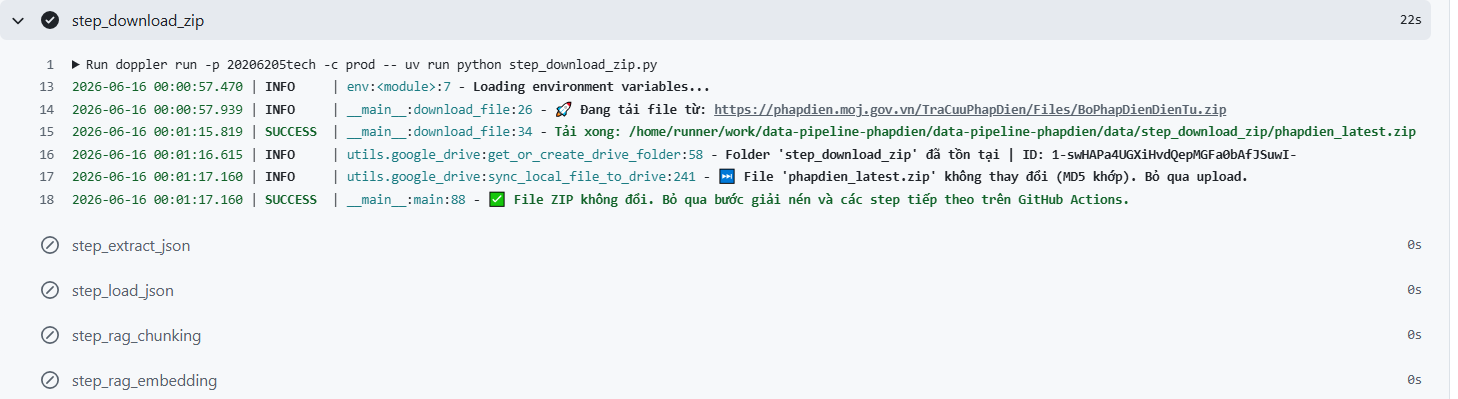
\includegraphics[width=0.95\textwidth]{pictures/data-pipeline-phapdien-step-download-zip-check-hash-skip-step.png}
\caption{Kiểm tra mã băm và bỏ qua bước tải nếu không có sự thay đổi dữ liệu}
\end{figure}
\end{itemize}

% \textbf{Giai đoạn Tiền xử lý Dữ liệu:}
\begin{itemize}
\item \texttt{step\_extract\_json} và \texttt{step\_load\_json}: Từ file \texttt{jsonData.js}, tiến hành bóc tách (parse) các biến cấu trúc dữ liệu để lấy danh sách chủ đề (\texttt{jdChuDe}), đề mục (\texttt{jdDeMuc}) và cây mục lục (\texttt{jdAllTree}), sau đó xuất ra định dạng JSON.

\begin{figure}[H]
\centering
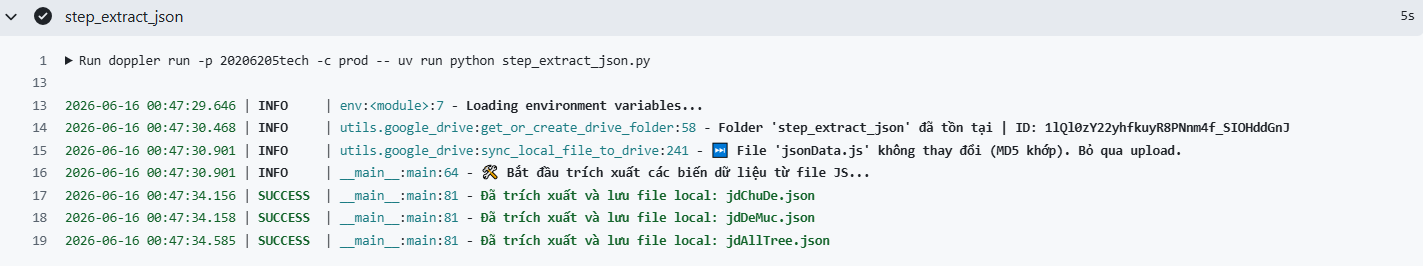
\includegraphics[width=0.95\textwidth]{pictures/data-pipeline-phapdien-step-extract-json.png}
\caption{Bóc tách biến cấu trúc dữ liệu và xuất ra file JSON}
\end{figure}

\begin{figure}[H]
\centering
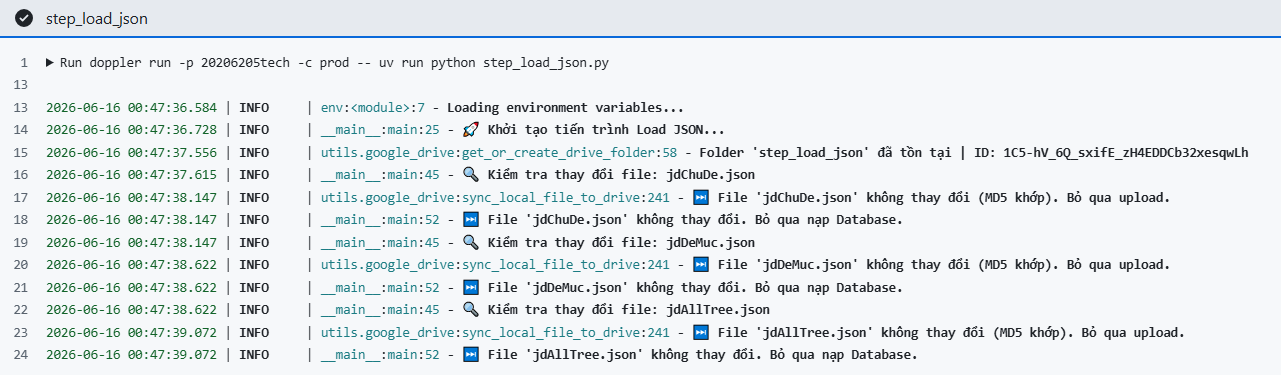
\includegraphics[width=0.95\textwidth]{pictures/data-pipeline-phapdien-step-load-json.png}
\caption{Nạp dữ liệu JSON vào hệ thống}
\end{figure}
\end{itemize}

% \textbf{Giai đoạn Tích hợp RAG Pipeline:}
\begin{itemize}
\item \texttt{step\_rag\_chunking}: Thực hiện đối chiếu từ cây mục lục (\texttt{jdAllTree}) với các thẻ bên trong từng file HTML chi tiết. Từ đó, bóc tách chính xác từng phần nội dung văn bản thành dạng JSON có các đoạn văn bản và siêu dữ liệu (Metadata).

\begin{figure}[H]
\centering
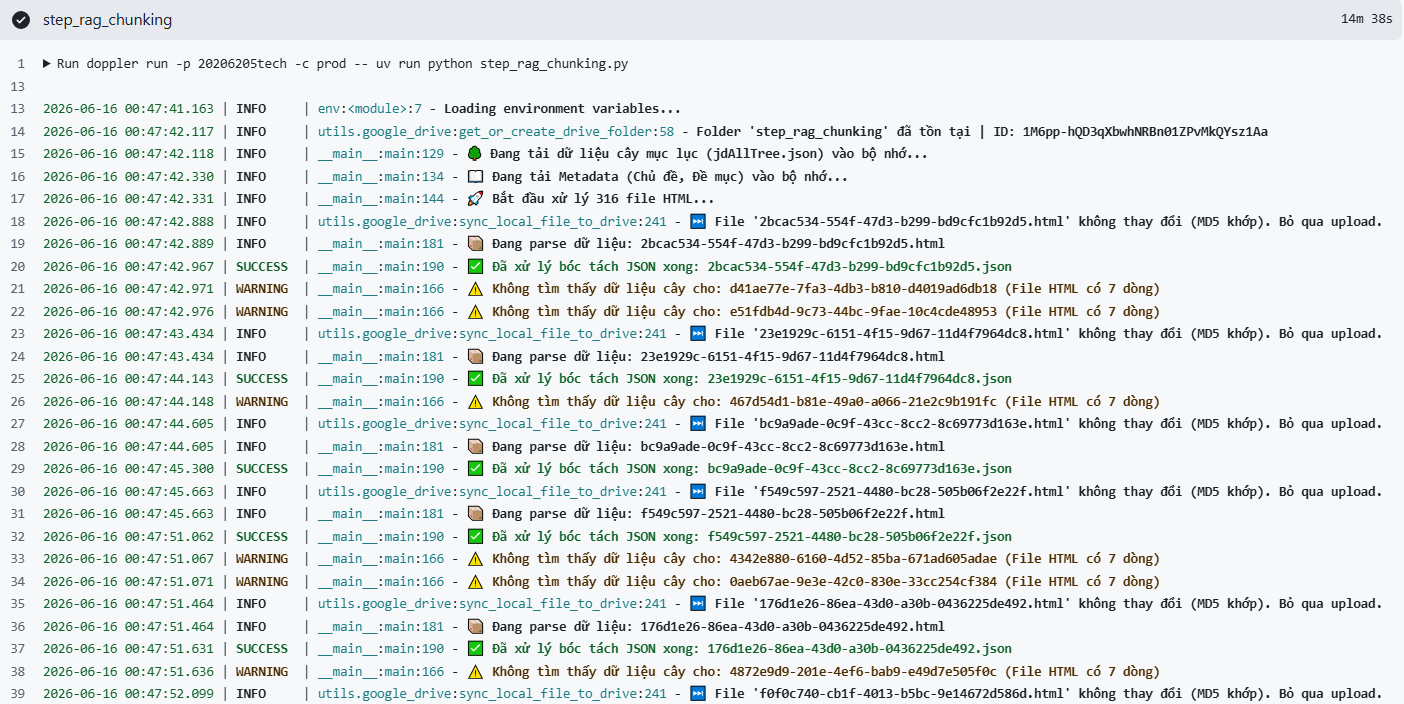
\includegraphics[width=0.8\textwidth]{pictures/data-pipeline-phapdien-step-rag-chunking.png}
\caption{Bóc tách và chia nhỏ nội dung văn bản theo cấu trúc mục lục}
\end{figure}

\item \texttt{step\_rag\_embedding}: Làm giàu ngữ cảnh bằng cách nối trực tiếp tên chủ đề và đề mục vào phần đầu của mỗi đoạn văn bản chunk. Sau đó, nội dung được đưa qua mô hình HuggingFace (\texttt{keepitreal/vietnamese-sbert}) để biến đổi thành các vector và lưu vào CSDL vector Qdrant.

\begin{figure}[H]
\centering
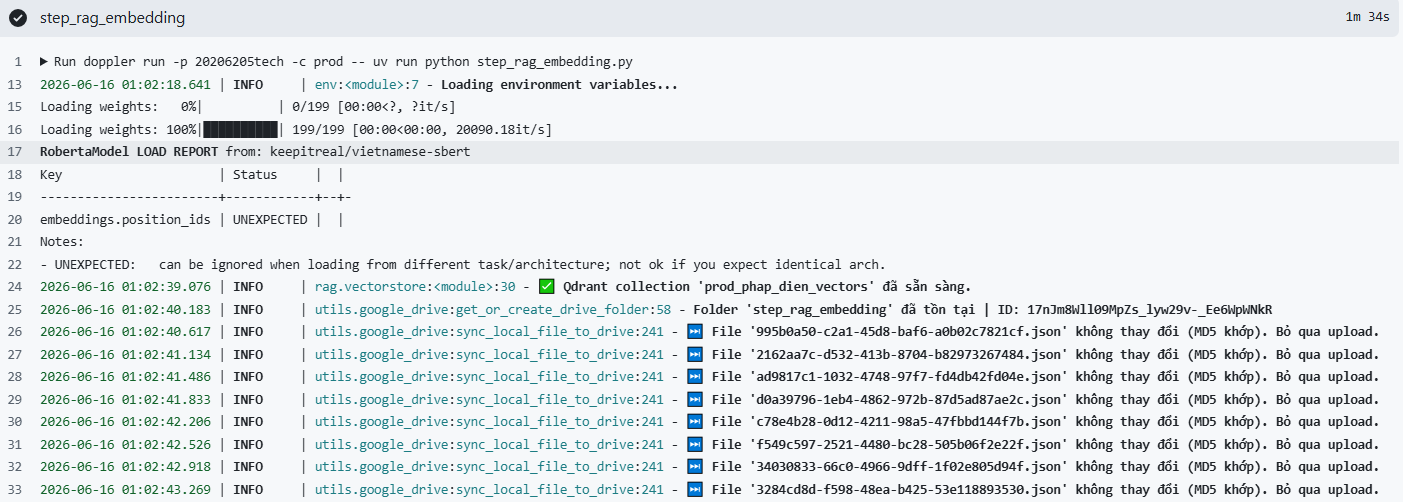
\includegraphics[width=0.95\textwidth]{pictures/data-pipeline-phapdien-step-rag-embedding.png}
\caption{Mô hình hóa dữ liệu dạng vector và lưu trữ vào Qdrant}
\end{figure}
\end{itemize}

\begin{figure}[H]
\centering
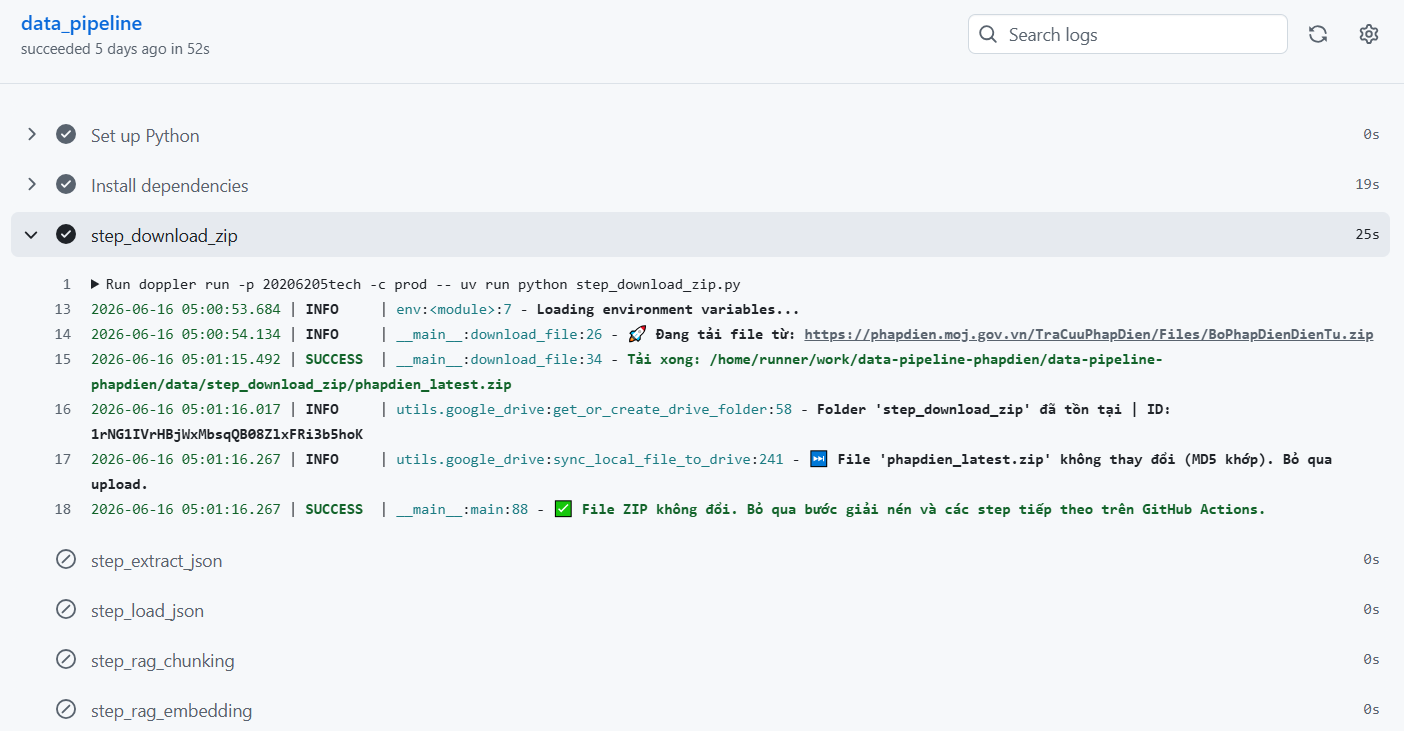
\includegraphics[width=0.95\textwidth]{pictures/github-action-PhapDien-v2.png}
\caption{So sánh mã băm để bỏ qua xử lý luồng dữ liệu Pháp Điển}
\end{figure}
